\usetikzlibrary{arrows,shapes}

\tikzstyle{inputNode}=[draw,circle,minimum size=10pt,inner sep=0pt]
\tikzstyle{stateTransition}=[->, thick]
\tikzstyle{hidden}=[draw,circle,minimum size=25pt,inner sep=0pt,fill=RoyalBlue!50]
\tikzstyle{output}=[draw,fill=blue!50,circle,minimum size=10pt,inner sep=0pt]

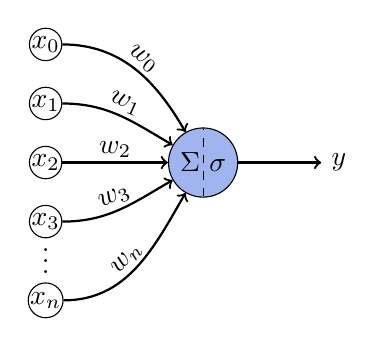
\begin{tikzpicture}
    \node[hidden] (x) at (0,0) {$\Sigma$ $\sigma$};

    \node[inputNode] (x0) at (-2, 1.5) {$\tiny x_0$};
    \node[inputNode] (x1) at (-2, 0.75) {$\tiny x_1$};
    \node[inputNode] (x2) at (-2, 0) {$\tiny x_2$};
    \node[inputNode] (x3) at (-2, -0.75) {$\tiny x_3$};
    \node[inputNode] (xn) at (-2, -1.75) {$\tiny x_n$};
    \node          (dots) at (-2, -1.15) {$\vdots$};

    \draw[stateTransition] (x0) to[out=0,in=120] node [midway, sloped, above=-2] {$w_0$} (x);
    \draw[stateTransition] (x1) to[out=0,in=150] node [midway, sloped, above=-2] {$w_1$} (x);
    \draw[stateTransition] (x2) to[out=0,in=180] node [midway, sloped, above=-2] {$w_2$} (x);
    \draw[stateTransition] (x3) to[out=0,in=210] node [midway, sloped, above=-2] {$w_3$} (x);
    \draw[stateTransition] (xn) to[out=0,in=240] node [midway, sloped, above=-2] {$w_n$} (x);
    \draw[stateTransition] (x) -- (1.5,0) node[right] {$y$};
    \draw[dashed] (0,-0.43) -- (0,0.43);
\end{tikzpicture}